\chapter{Supplementary Material} \label{app:math}

\section{Verifying \pp for Sufficiency} \label{sec:sufficiency}
% Reminder to swap out "calibration" for "sufficiency"
% Note: Google testing for conditional independence via correlation tests

Sufficiency requires that conditional on the predicted status, the protected attribute is independent from the true status. In our setting, all three variables (protected attribute, prediction, and true status) are continuous, which complicates both statistical and graphical checks. Statistically, verifying conditional independence for continuous variables is a hard problem \citep{bergsma_testing_2004}. Graphically, \citet{barocas_fairness_2018} introduce the approach of plotting accuracy curves for each predicted group separately. However, because the protected attribute in our case is continuous for each grid cell, this approach also does not work.

To provide initial evidence that \pp satisfies sufficiency, we bin grid cells by predicted intensity and calculate the correlation between number of actual crimes and demographic (percentage black or white) for the grid cells in each bin. Within each bin of cells of similar predicted intensity, we should see no correlation (close to 0.0) between the number of actual crimes and the percentage black/white. We repeat this procedure for each day that was predicted in the test set, and plot each observed correlation as a separate point (so there may be more than one point for the same bin). Not every bin on each day has enough grid cells (more than two) to perform Pearson's r meaningfully; those points are omitted from the graph.

\autoref{fig:sufficiency} shows the scatter plot of these results. If \pp is calibrated, we would expect most of the y-values to be close to zero, which is what we observe. We see instead that for some days, there is indeed a strong correlation between demographics and number of crimes, even after conditioning on predicted intensity. Further research is necessary to verify these results and, if the results are verified, interrogate their implications.
% Results from the same test day in 2015 have the same color. Reassuringly, we do not see any clustering based on color. If we did, we might still be concerned about the calibration of \pp, since on

\begin{figure}[bth]
    \myfloatalign
    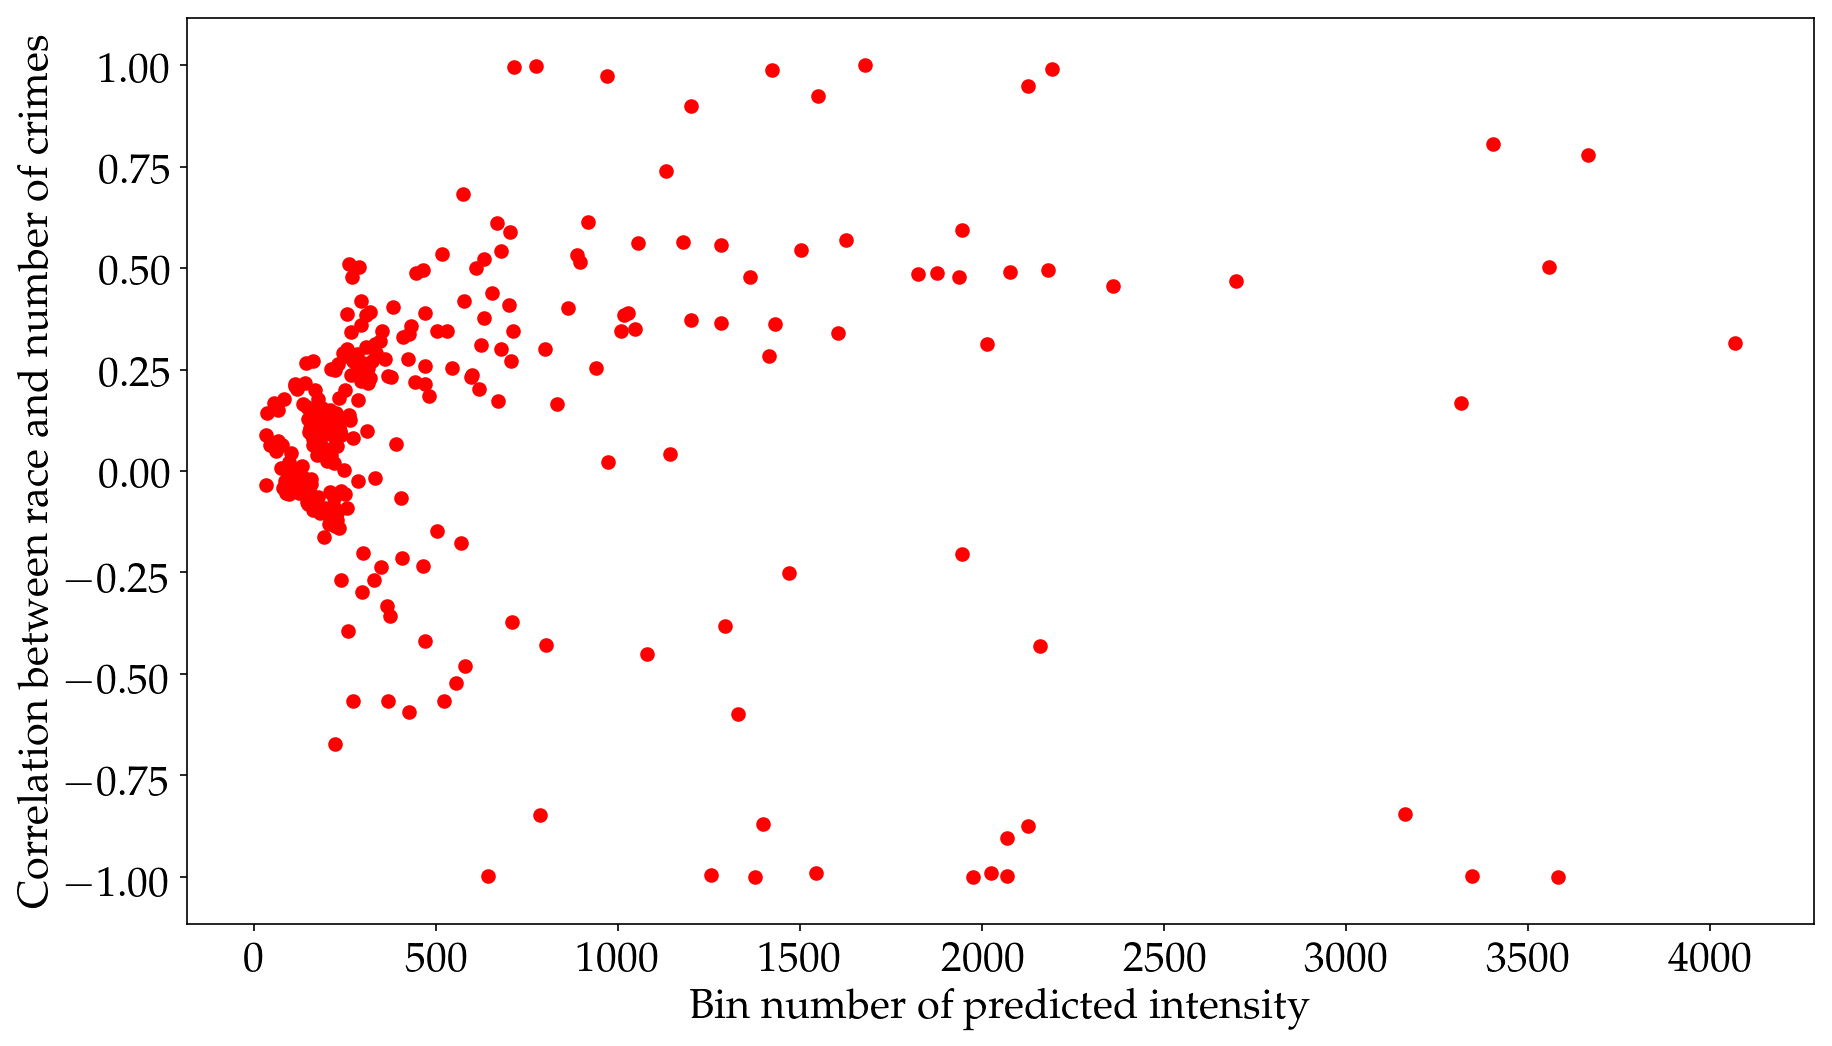
\includegraphics[width=.9\linewidth]{gfx/CalibrationScatter.png}
    \caption{Verifying that \pp satisfies sufficiency}
    \label{fig:sufficiency}
\end{figure}

\pagebreak
\section{Proof of Incompatibility from \autoref{ch:fairness_primer}} \label{proof:ch_3}

The following proves the incompatibility of these two fairness notions in real-world situations:
\begin{align}
\intertext{Equalized Odds:}
p(\hat{Y} \mid Y, A = 1) &= p(\hat{Y} \mid Y, A = 0) \label{eq:eq_op}\\
\intertext{Equal Desert (Sufficiency):}
p(A \mid Y = 1) &= p(A \mid \hat{Y} = 1) \label{eq:def_other1}\\
p(A \mid Y = 0) &= p(A \mid \hat{Y} = 0) \label{eq:def_other2}
\end{align}
Equation~\ref{eq:def_other1} says, "the percentage of crime group $A$ is responsible for equals the percentage of group $A$ in the locations visited." The proof proceeds by showing that if all of the above equations are true, edge-case conditions must also be true (and so in general, not all of the above equations can be true).\footnote{The form of this proof closely resembles the proofs found in \citet{barocas_fairness_2018}.} Start by applying the law of total probability to the right-hand side of equation~\ref{eq:def_other1}.
\begin{align}
p(A \mid \hat{Y} = 1) &= \sum_{Y} p(A \mid Y, \hat{Y} = 1) \; p(Y \mid \hat{Y} = 1) \label{eq:proof_line1}\\
&= \sum_{Y} p(A \mid Y) \; p(Y \mid \hat{Y} = 1)
\end{align}
The second line holds from applying equation~\ref{eq:eq_op}, since the protected category $A$ will be independent from predictions $\hat{Y}$ given the true status $Y$.
\begin{align}
p(A &\mid \hat{Y} = 1)\\
&= p(A \mid Y = 0)p(Y = 0 \mid \hat{Y} = 1) + p(A \mid Y = 1)p(Y = 1 \mid \hat{Y} = 1)\\
&= p(A \mid Y = 0)p(Y = 0 \mid \hat{Y} = 1) + p(A \mid Y = 1)(1 - p(Y = 0 \mid \hat{Y} = 1))\\
&= p(A \mid \hat{Y} = 0)p(Y = 0 \mid \hat{Y} = 1) + p(A \mid \hat{Y} = 1)(1 - p(Y = 0 \mid \hat{Y} = 1))
\end{align}
Here, we make use of the assumptions in equations~\ref{eq:def_other1} and
\ref{eq:def_other2}. Now dividing both sides by $p(A \mid \hat{Y} = 1)$:
\begin{align}
1 &= \frac{p(A \mid \hat{Y} = 0)}{p(A \mid \hat{Y} = 1)}p(Y = 0 \mid \hat{Y} = 1) + 1 - p(Y = 0 \mid \hat{Y} = 1)\\
0 &= p(Y = 0 \mid \hat{Y} = 1) \left(\frac{p(A \mid \hat{Y} = 0)}{p(A \mid \hat{Y} = 1)} - 1\right)
\end{align}
So either $p(Y = 0 \mid \hat{Y} = 1) = 0$ or $p(A \mid \hat{Y} = 0) = p(A \mid
\hat{Y} = 1)$. The first condition states that the algorithm has 100\%
precision. By conditioning on $\hat{Y} = 0$ instead of $\hat{Y} = 1$ in
equation~\ref{eq:proof_line1}, we also obtain the implication that $p(Y = 0
\mid \hat{Y} = 0) = 0$. In other words, this first condition states that the
policing algorithm must be 100\% accurate. The second condition, because of our
assumptions in in equations~\ref{eq:def_other1} and \ref{eq:def_other2}, can
also be rewritten as: $p(A \mid Y = 0) = p(A \mid Y = 1)$. It is rarely the case that the demographics of those who do commit crimes and those who do not are identical however.

Because \autoref{eq:eq_op}, \autoref{eq:def_other1}, and \autoref{eq:def_other2} together imply edge case conditions, we can conclude that in general all three cannot hold simultaneously.
